%%%%%%%%%%%%%%%%%%%%%%%%%%%%%%%%%%%%
% 配布用ハンドアウト（解答なし）
% コンパイルコマンド: lualatex chp8_handout.tex
%%%%%%%%%%%%%%%%%%%%%%%%%%%%%%%%%%%%

\documentclass[slidestop,compress,mathserif,handout]{beamer}

% 解答を非表示にする
\newcommand{\soln}[1]{ }
\newcommand{\solnGr}[1]{ }

% 4スライドを1ページに印刷する設定
\usepackage{pgfpages}
\pgfpagesuselayout{4 on 1}[a4paper,landscape,border shrink=5mm]

%%%%%%%%%%%%%%%%%%%%%%%%%%%%%%%%%%%%
% 日本語サポート（LuaLaTeX使用）
%%%%%%%%%%%%%%%%%%%%%%%%%%%%%%%%%%%%

\usepackage{luatexja}
\usepackage{luatexja-fontspec}

%%%%%%%%%%%%%%%%%%%%%%%%%%%%%%%%%%%%
% スタイル
%%%%%%%%%%%%%%%%%%%%%%%%%%%%%%%%%%%%

\input{../lec_style_JP}

% 配布用：練習問題の正解を通常アイテムとして表示（オーバーレイなし）
\renewcommand{\solnMult}[1]{\item #1}


%%%%%%%%%%%%%%%%%%%%%%%%%%%%%%%%%%%%
% プリアンブル
%%%%%%%%%%%%%%%%%%%%%%%%%%%%%%%%%%%%

\title[第8章：線形回帰入門]{第8章：線形回帰入門}
\author{OpenIntro Statistics 第4版（日本語版）}
\institute{$\:$ \\ {\footnotesize 原著スライド：Mine \c{C}etinkaya-Rundel（OpenIntro）\\
\webLink{http://creativecommons.org/licenses/by-sa/3.0/us/}{CC BY-SA ライセンス}のもと使用・翻訳。\\
一部の画像はフェアユース（教育目的）に基づき使用。}}
\date{}

%%%%%%%%%%%%%%%%%%%%%%%%%%%%%%%%%%%%
% ドキュメント開始
%%%%%%%%%%%%%%%%%%%%%%%%%%%%%%%%%%%%

\begin{document}


%%%%%%%%%%%%%%%%%%%%%%%%%%%%%%%%%%%%
% タイトルページ
%%%%%%%%%%%%%%%%%%%%%%%%%%%%%%%%%%%%

{
\addtocounter{framenumber}{-1}
{\removepagenumbers
\usebackgroundtemplate{
\includegraphics[width=\paperwidth]{../OpenIntro_Grid_4_3-01.jpg}}
\begin{frame}

\hfill 
\includegraphics[width=20mm]{../oiLogo_highres}

\titlepage

\end{frame}
}
}


%%%%%%%%%%%%%%%%%%%%%%%%%%%%%%%%%%%%
% 各節
%%%%%%%%%%%%%%%%%%%%%%%%%%%%%%%%%%%%

%%%%%%%%%%%%%%%%%%%%%%%%%%%%%%%%%%%%

\section{直線の当てはめ、残差、相関}

%%%%%%%%%%%%%%%%%%%%%%%%%%%%%%%%%%%%

\subsection{データへの直線の当てはめ}

%%%%%%%%%%%%%%%%%%%%%%%%%%%%%%%%%%%%

\begin{frame}
\frametitle{数値変数のモデル化}

本節では、2つの数値変数間の関係を定量化する方法と、数値または質的な説明変数を用いて数値の目的変数をモデル化する方法を学ぶ。

\end{frame}

%%%%%%%%%%%%%%%%%%%%%%%%%%%%%%%%%%%%

\begin{frame}
\frametitle{貧困率と高校卒業率}

下の\hl{散布図}は、米国全50州とワシントンDCの高校卒業率と、貧困ライン（2012年時点で4人家族の年収23,050ドル未満）以下で生活する住民の割合との関係を示している。

\twocol{0.55}{0.45}{
\begin{center}
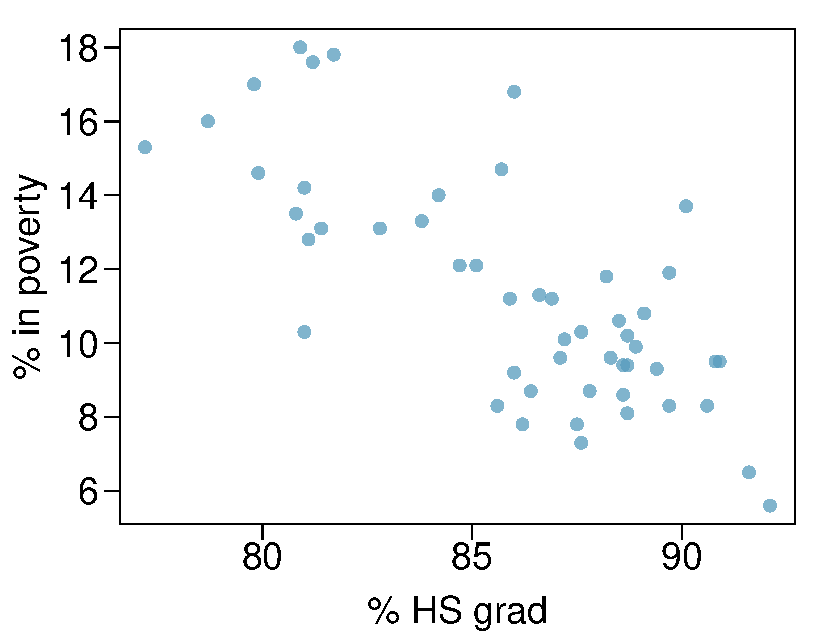
\includegraphics[width=\textwidth]{8-1_linefit_res_corr/figures/poverty/poverty_hsgrad}
\end{center}
}
{
\dq{目的変数は？}
\soln{貧困率（\%）}
\dq{説明変数は？}
\soln{高校卒業率（\%）}
\dq{関係は？}
\soln{線形、負の相関、中程度の強さ}
}

\end{frame}

%%%%%%%%%%%%%%%%%%%%%%%%%%%%%%%%%%%

\subsection{線形回帰を用いた貧困率の予測}

%%%%%%%%%%%%%%%%%%%%%%%%%%%%%%%%%%%

\begin{frame}

米国の高校卒業率から貧困率を予測する線形モデルは次のとおりである：

\[ \hat{poverty} = 64.78 - 0.62 \times HS_{grad} \]

「ハット（$\hat{\:}$）」は推定値であることを示す。

\end{frame}

%%%%%%%%%%%%%%%%%%%%%%%%%%%%%%%%%%%

\begin{frame}

\dq{ジョージア州の高校卒業率は85.1\%である。このモデルは同州の貧困率をどのように予測するか？}

\[ 64.78 - 0.62 \times 85.1 = 12.018 \]

\end{frame}

%%%%%%%%%%%%%%%%%%%%%%%%%%%%%%%%%%%

\subsection{直線の目視確認}

%%%%%%%%%%%%%%%%%%%%%%%%%%%%%%%%%%%

\begin{frame}
\frametitle{直線の目視確認}

\twocol{0.3}{0.7}
{
\pq{貧困率と高校卒業率の線形関係に最もよく当てはまる直線はどれか。1つ選べ。}
\soln{\only<2>{\orange{
(a)
}}}
}
{
\begin{center}

\includegraphics[width=\textwidth]{8-2_least_square_reg/figures/poverty/poverty_hsgrad_manylines}
\end{center}
}
\end{frame}

%%%%%%%%%%%%%%%%%%%%%%%%%%%%%%%%%%%

\subsection{残差}

%%%%%%%%%%%%%%%%%%%%%%%%%%%%%%%%%%%

\begin{frame}
\frametitle{残差}

\hl{残差}とはモデルの当てはめから残ったものである：データ = 当てはめ値 + 残差

\begin{center}
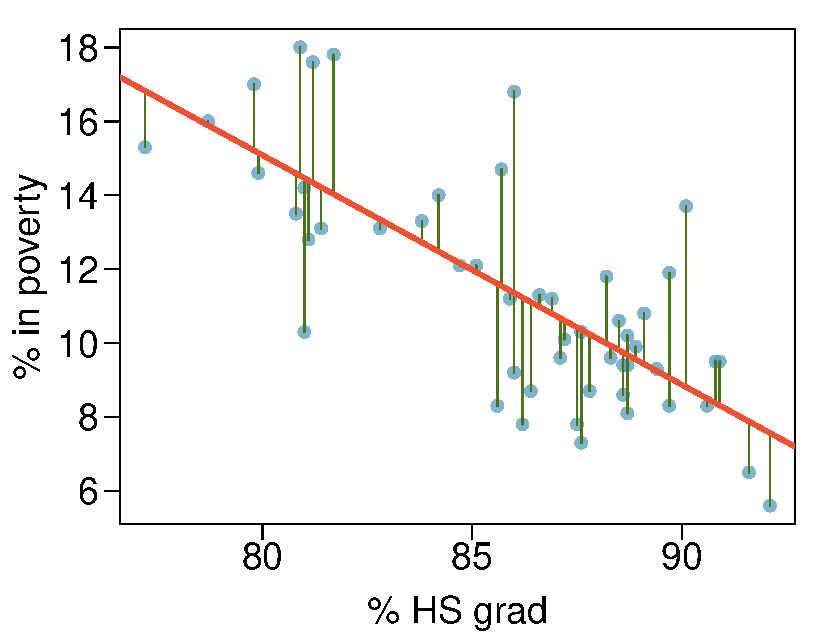
\includegraphics[width=0.8\textwidth]{8-2_least_square_reg/figures/poverty/poverty_hsgrad_res}
\end{center}

\end{frame}

%%%%%%%%%%%%%%%%%%%%%%%%%%%%%%%%%%

\begin{frame}
\frametitle{残差（続き）}

\formula{残差}{
残差は観測値（$y_i$）と予測値$\hat{y}_i$との差である。
\[ e_i = y_i - \hat{y}_i \]
}
\vspace{-0.5cm}
\twocol{0.6}{0.4}
{
\begin{center}
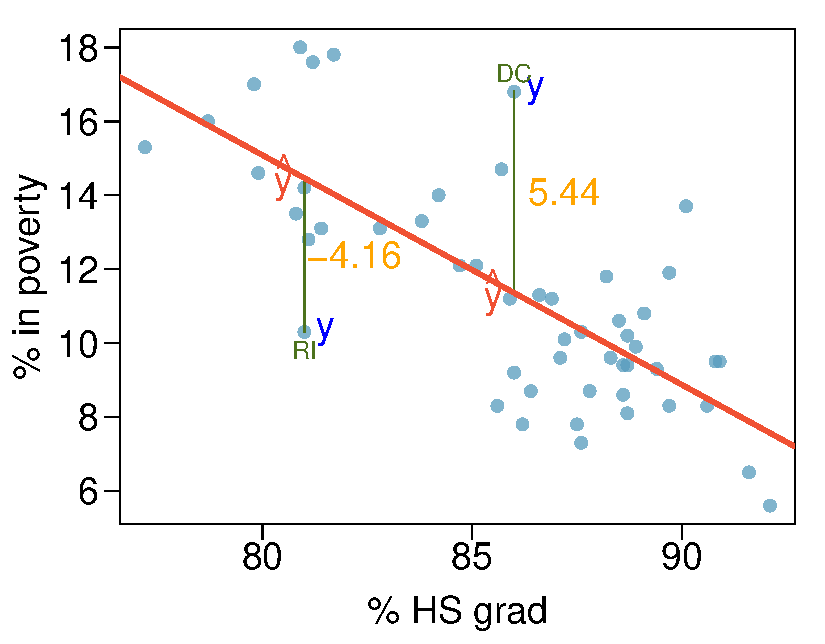
\includegraphics[width=\textwidth]{8-2_least_square_reg/figures/poverty/poverty_hsgrad_res_text}
\end{center}
}
{
\begin{itemize}
\item ワシントンDCの貧困率は予測値より5.44\%高い。
\item ロードアイランド州の貧困率は予測値より4.16\%低い。
\end{itemize}
}


\end{frame}

%%%%%%%%%%%%%%%%%%%%%%%%%%%%%%%%%%

\subsection{相関による線形関係の記述}

%%%%%%%%%%%%%%%%%%%%%%%%%%%%%%%%%%%

\begin{frame}
\frametitle{関係の定量化}

\begin{itemize}

\item \hl{相関}は2つの変数間の\orange{線形}な関連の強さを表す。

\item $-1$（完全な負の相関）から$+1$（完全な正の相関）の値をとる。

\item 値が0の場合、線形な関連がないことを示す。

\end{itemize}

\end{frame}

%%%%%%%%%%%%%%%%%%%%%%%%%%%%%%%%%%%

\begin{frame}
\frametitle{相関の推測}

\pq{貧困率と高校卒業率の相関として最もよい推測はどれか？}
\twocol{0.4}{0.6}
{
\begin{enumerate}[(a)]
\item 0.6
\solnMult{-0.75}
\item -0.1
\item 0.02
\item -1.5
\end{enumerate}
}
{
\begin{center}
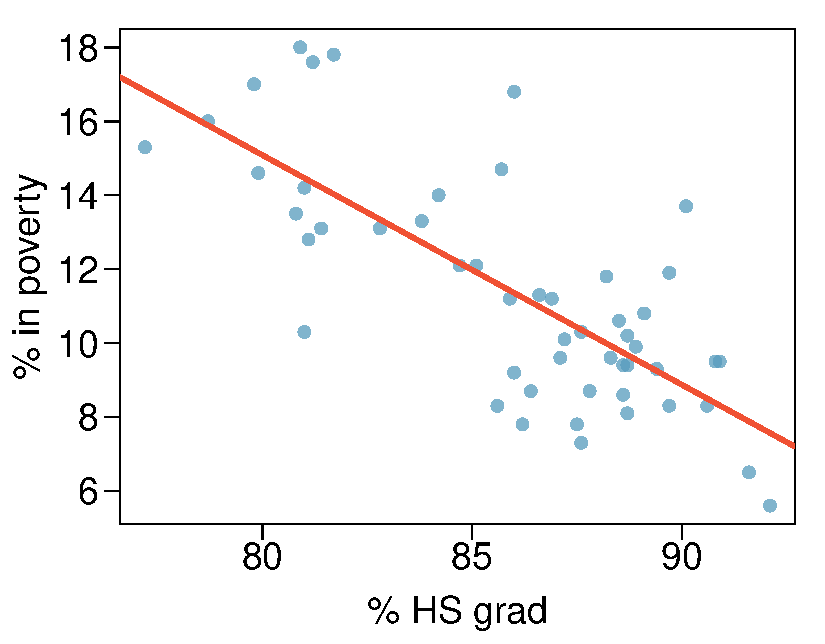
\includegraphics[width=\textwidth]{8-1_linefit_res_corr/figures/poverty/poverty_hsgrad_line}
\end{center}
}

\end{frame}

%%%%%%%%%%%%%%%%%%%%%%%%%%%%%%%%%%

\begin{frame}
\frametitle{相関の推測}

\pq{貧困率と「夫なし女性世帯主」の割合の相関として最もよい推測はどれか？}

\twocol{0.4}{0.6}
{
\begin{enumerate}[(a)]
\item 0.1
\item -0.6
\item -0.4
\item 0.9
\solnMult{0.5}
\end{enumerate}
}
{
\begin{center}
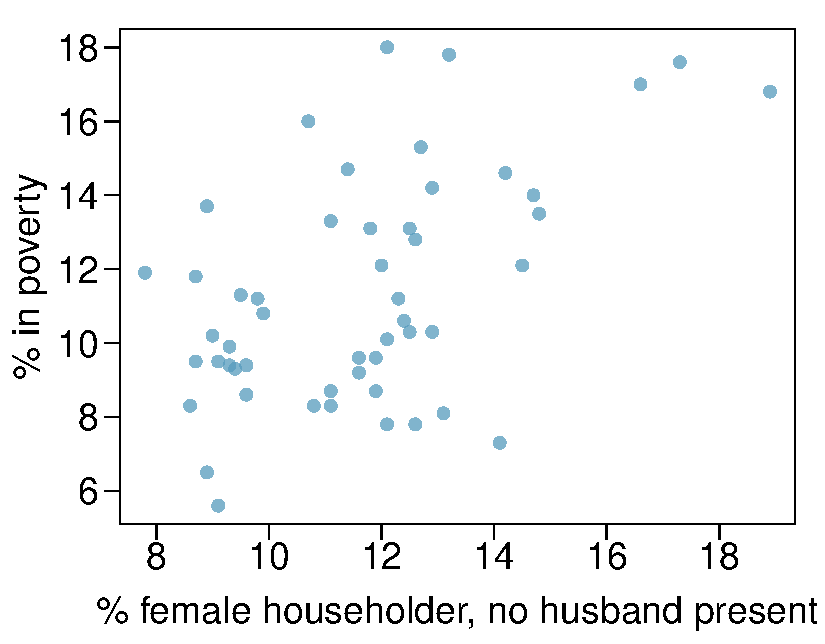
\includegraphics[width=\textwidth]{8-1_linefit_res_corr/figures/poverty/poverty_nohusband}
\end{center}
}

\end{frame}

%%%%%%%%%%%%%%%%%%%%%%%%%%%%%%%%%%

\begin{frame}
\frametitle{相関の評価}

\pq{以下のうち、最も強い相関（相関係数が+1または-1に最も近い）を持つのはどれか？}

\twocol{0.8}{0.2}
{
\begin{center}
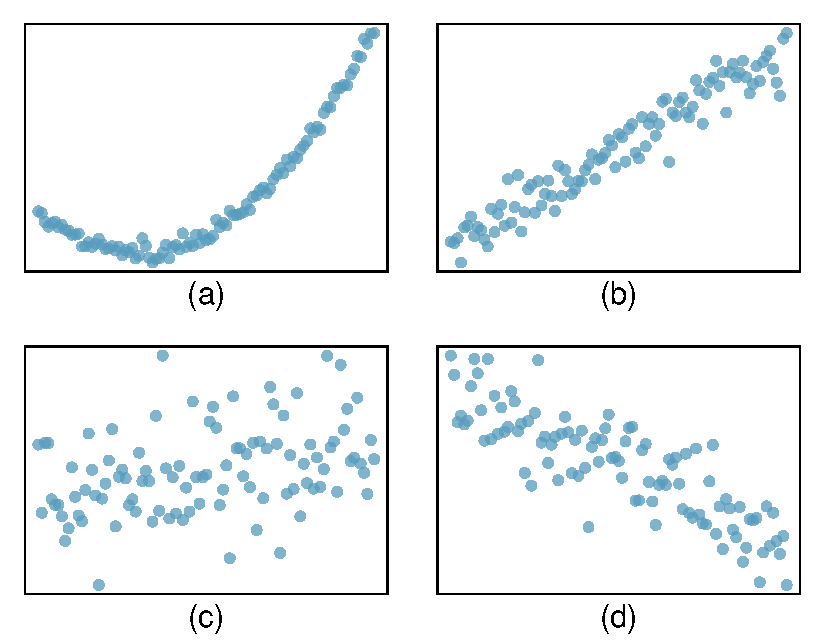
\includegraphics[width=0.75\textwidth]{8-1_linefit_res_corr/figures/cor/cor}
\end{center}
}
{
\soln{\only<2>{\orange{
(b) $\rightarrow$ 相関は\underline{線形}な関連を意味する
}}}
}

\end{frame}

%%%%%%%%%%%%%%%%%%%%%%%%%%%%%%%%%%%%

\section{最小二乗法による直線の当てはめ}

%%%%%%%%%%%%%%%%%%%%%%%%%%%%%%%%%%%%

\subsection{最良の直線を見つけるための客観的な基準}

%%%%%%%%%%%%%%%%%%%%%%%%%%%%%%%%%%%

\begin{frame}
\frametitle{最良の直線を見つけるための客観的な基準}

\begin{itemize}

\item 残差が小さい直線を求める：
\begin{enumerate}
\item 方法1：残差の絶対値の和を最小化する
\[ |e_1| + |e_2| + \cdots + |e_n| \]
\item 方法2：残差の二乗和を最小化する――\hl{最小二乗法}
\[ e_1^2 + e_2^2 + \cdots + e_n^2 \]
\end{enumerate}

\item なぜ最小二乗法か？
\begin{enumerate}
\item 最も広く使われている
\item 手計算およびソフトウェアによる計算が容易
\item 多くの場面で、2倍の大きさの残差は通常2倍以上に悪いとみなされる
\end{enumerate}

\end{itemize}

\end{frame}

%%%%%%%%%%%%%%%%%%%%%%%%%%%%%%%%%%

\begin{frame}
\frametitle{最小二乗直線}

\[ \mathhl{ \hat{y} = \beta_0 + \beta_1 x } \]

\begin{itemize}
\item $\hat{y}$：目的変数$y$の予測値
\item $\beta_0$：切片（母数）
\begin{itemize}
\item $b_0$：切片（点推定量）
\end{itemize}
\item $\beta_1$：傾き（母数）
\begin{itemize}
\item $b_1$：傾き（点推定量）
\end{itemize}
\item $x$：説明変数
\end{itemize}

\end{frame}

%%%%%%%%%%%%%%%%%%%%%%%%%%%%%%%%%%

\subsection{最小二乗直線の条件}

%%%%%%%%%%%%%%%%%%%%%%%%%%%%%%%%%%%

\begin{frame}
\frametitle{最小二乗直線の条件}

\begin{enumerate}

\item 線形性

\item 残差がほぼ正規分布に従う

\item 等分散性（一定のばらつき）

\end{enumerate}

\end{frame}

%%%%%%%%%%%%%%%%%%%%%%%%%%%%%%%%%%

\begin{frame}
\frametitle{条件（1）：線形性}

\begin{itemize}

\item 説明変数と目的変数の関係は線形でなければならない。

\item 非線形な関係へのモデル当てはめ手法も存在するが、本講義の範囲を超える。この話題に興味があれば、\href{http://www.openintro.org/download.php?file=os2_extra_nonlinear_relationships&referrer=/stat/textbook.php}{openintro.orgのオンライン補足資料}で新しい手法を学べる。

\item 散布図または\hl{残差プロット}を用いて確認する。

\end{itemize}

\begin{center}
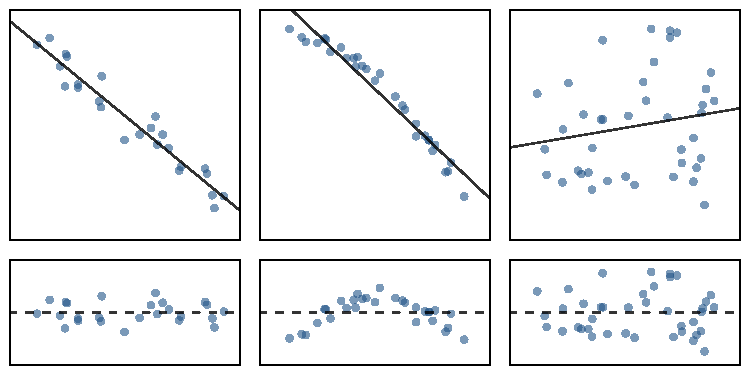
\includegraphics[width=0.7\textwidth]{8-2_least_square_reg/figures/sampleLinesAndResPlots/sampleLinesAndResPlots}
\end{center}

\end{frame}

%%%%%%%%%%%%%%%%%%%%%%%%%%%%%%%%%%

\begin{frame}[shrink=15]
\frametitle{残差プロットの見方}

\twocol{0.5}{0.5}
{
\begin{center}
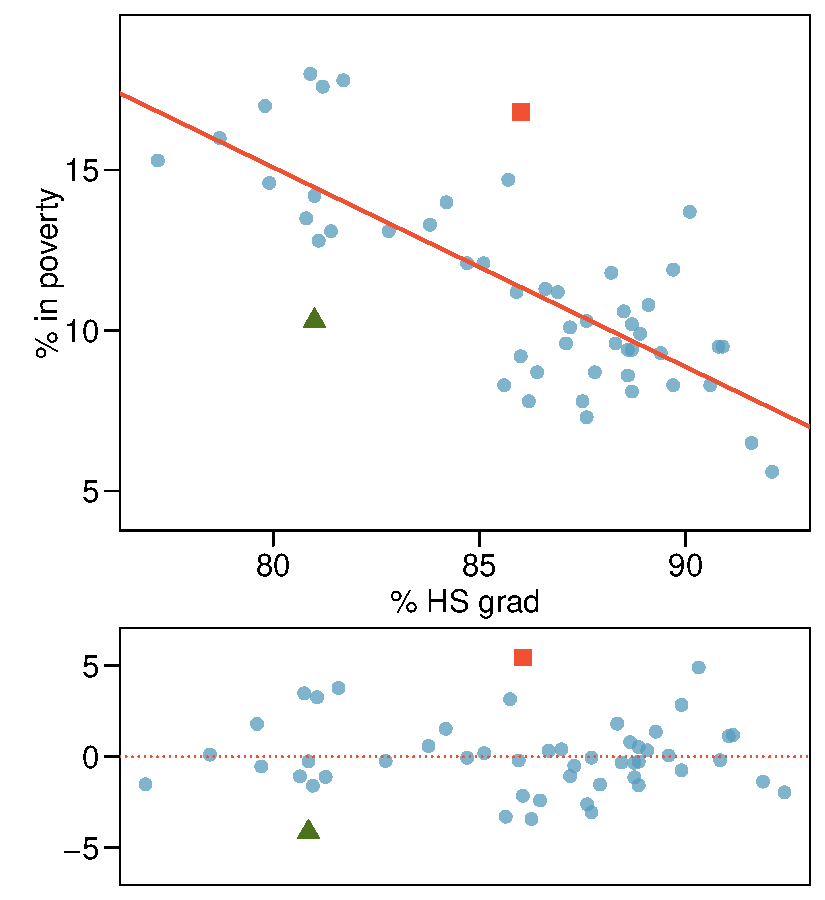
\includegraphics[width=\textwidth]{8-2_least_square_reg/figures/poverty/poverty_hsgrad_resplot}
\end{center}
}
{
{\small
\green{{\large $\blacktriangle$}} \hl{RI（ロードアイランド州）:}
\begin{align*}
\%~HS~grad &= 81,\quad \%~in~poverty = 10.3 \\
\widehat{\%~in~poverty} &= 64.68 - 0.62 \times 81 = 14.46 \\
e &= 10.3 - 14.46 = \green{$-4.16$}
\end{align*}
\textcolor{red}{{\normalsize $\blacksquare$}} \hl{DC（ワシントンDC）:}
\begin{align*}
\%~HS~grad &= 86,\quad \%~in~poverty = 16.8 \\
\widehat{\%~in~poverty} &= 64.68 - 0.62 \times 86 = 11.36 \\
e &= 16.8 - 11.36 = \textcolor{red}{5.44}
\end{align*}
}
}

\end{frame}


%%%%%%%%%%%%%%%%%%%%%%%%%%%%%%%%%%

\begin{frame}
\frametitle{条件（2）：残差がほぼ正規分布に従う}

\begin{itemize}

\item 残差はほぼ正規分布に従う必要がある。

\item データの傾向から外れた異常な観測値がある場合、この条件が満たされないことがある。

\item ヒストグラムを用いて確認する。

\end{itemize}

\begin{center}
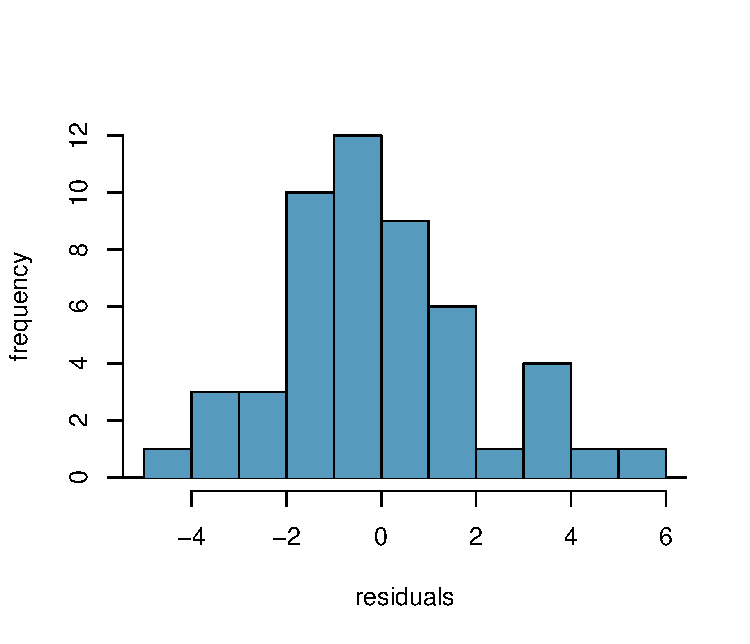
\includegraphics[width=0.5\textwidth]{8-2_least_square_reg/figures/poverty/normal_res}
\end{center}

\end{frame}

%%%%%%%%%%%%%%%%%%%%%%%%%%%%%%%%%%

\begin{frame}
\frametitle{条件（3）：等分散性（一定のばらつき）}

\twocol{0.5}{0.5}
{
\begin{center}
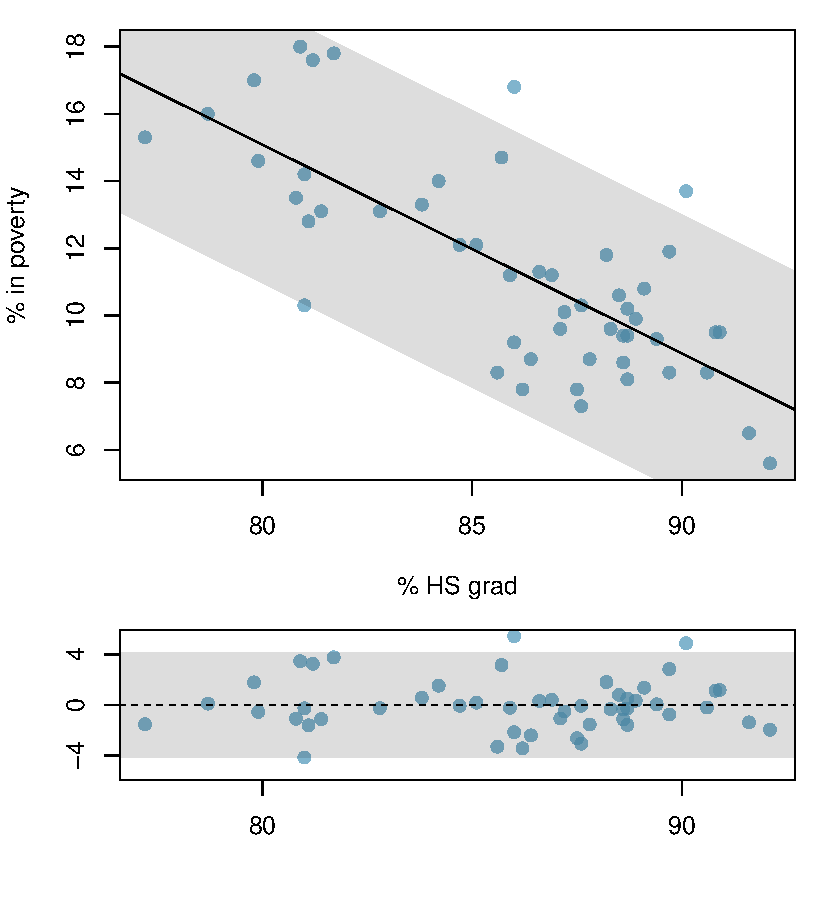
\includegraphics[width=\textwidth]{8-2_least_square_reg/figures/poverty/poverty_hsgrad_tube}
\end{center}
}
{
\begin{itemize}

\item 最小二乗直線の周りの点のばらつきはおおむね一定でなければならない。

\item これは、0の線の周りの残差のばらつきもおおむね一定であることを意味する。

\item \hl{等分散性（homoscedasticity）}とも呼ばれる。

\item 残差プロットを用いて確認する。

\end{itemize}
}


\end{frame}

%%%%%%%%%%%%%%%%%%%%%%%%%%%%%%%%%%

\begin{frame}
\frametitle{条件の確認}

\twocol{0.5}{0.5}
{
\pq{この線形モデルが明らかに違反している条件はどれか？}
\begin{enumerate}[(a)]
\item 等分散性
\solnMult{線形関係}
\item 正規残差
\item 極端な外れ値がない
\end{enumerate}
}
{
\begin{center}
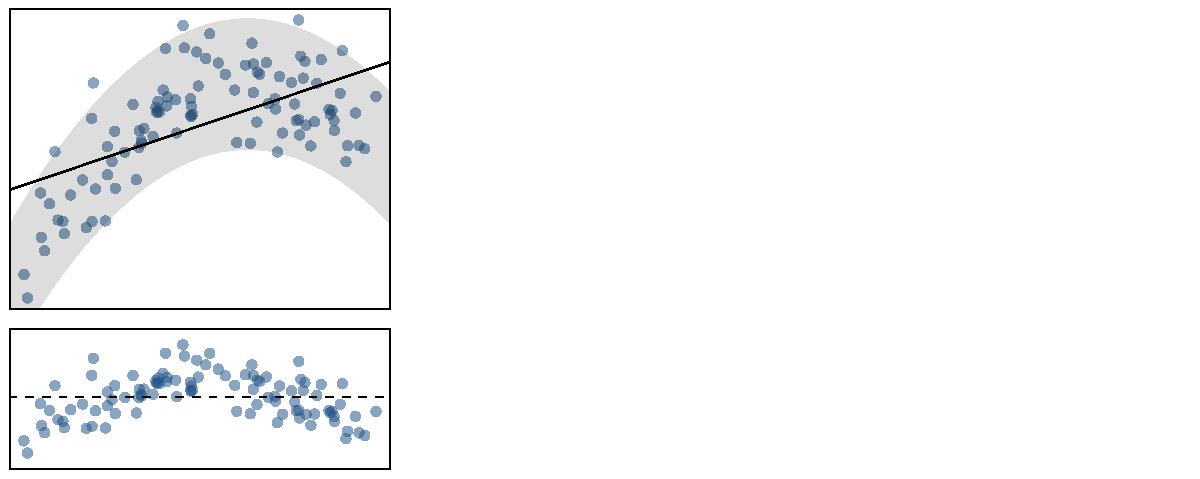
\includegraphics[width=\textwidth]{8-2_least_square_reg/figures/problems/nonlinear}
\end{center}
}

\end{frame}

%%%%%%%%%%%%%%%%%%%%%%%%%%%%%%%%%%

\begin{frame}
\frametitle{条件の確認}

\twocol{0.5}{0.5}
{
\pq{この線形モデルが明らかに違反している条件はどれか？}
\begin{enumerate}[(a)]
\solnMult{等分散性}
\item 線形関係
\item 正規残差
\item 極端な外れ値がない
\end{enumerate}
}
{
\begin{center}
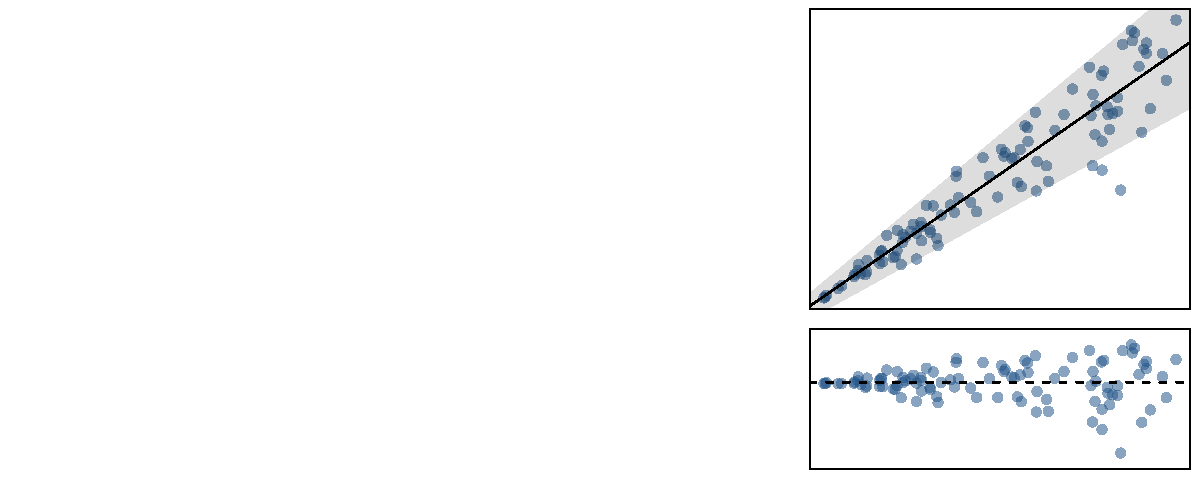
\includegraphics[width=\textwidth]{8-2_least_square_reg/figures/problems/heteroscedastic}
\end{center}
}

\end{frame}

%%%%%%%%%%%%%%%%%%%%%%%%%%%%%%%%%%%

\subsection{最小二乗直線の求め方}

%%%%%%%%%%%%%%%%%%%%%%%%%%%%%%%%%%%

\begin{frame}
\frametitle{与えられたデータ}

\twocol{0.5}{0.5}
{
\begin{center}

\includegraphics[width=0.7\linewidth]{8-2_least_square_reg/figures/poverty/poverty_hsgrad}
\end{center}
}
{
{\scriptsize
\begin{tabular}{l r r}
\hline
		& \shortstack[r]{高校卒業率\\（\%）}	& \shortstack[r]{貧困率\\（\%）} \\
		& $(x)$			& $(y)$ \\
\hline
平均	& $\bar{x} = 86.01$	& $\bar{y} = 11.35$  \\
標準偏差	& $s_x = 3.73$		& $s_y = 3.1$ \\
\hline
		& 相関		& $R = -0.75$ \\
\hline
\end{tabular}
}
}

\end{frame}

%%%%%%%%%%%%%%%%%%%%%%%%%%%%%%%%%%

\subsection{回帰モデルのパラメータ推定値の解釈}

%%%%%%%%%%%%%%%%%%%%%%%%%%%%%%%%%%

\begin{frame}
\frametitle{傾き}

\formula{傾き}
{回帰の傾きは次の式で計算できる：
\[ b_1 = \frac{s_y}{s_x} R \]
}

\hl{具体的には…}
\[ b_1 = \frac{3.1}{3.73} \times (-0.75) = -0.62 \]

$\:$ \\
\hl{解釈} \\
高校卒業率が1\%ポイント上昇するごとに、貧困率は平均的に0.62\%ポイント低下すると予測される。

\end{frame}

%%%%%%%%%%%%%%%%%%%%%%%%%%%%%%%%%%

\begin{frame}
\frametitle{切片}

\formula{切片}
{切片は回帰直線が$y$軸と交わる点である。回帰直線は常に$(\bar{x},\bar{y})$を通るという性質を用いて計算する：
\[ b_0 = \bar{y} - b_1 \bar{x} \]
}

\twocol{0.55}{0.45}
{
\begin{center}
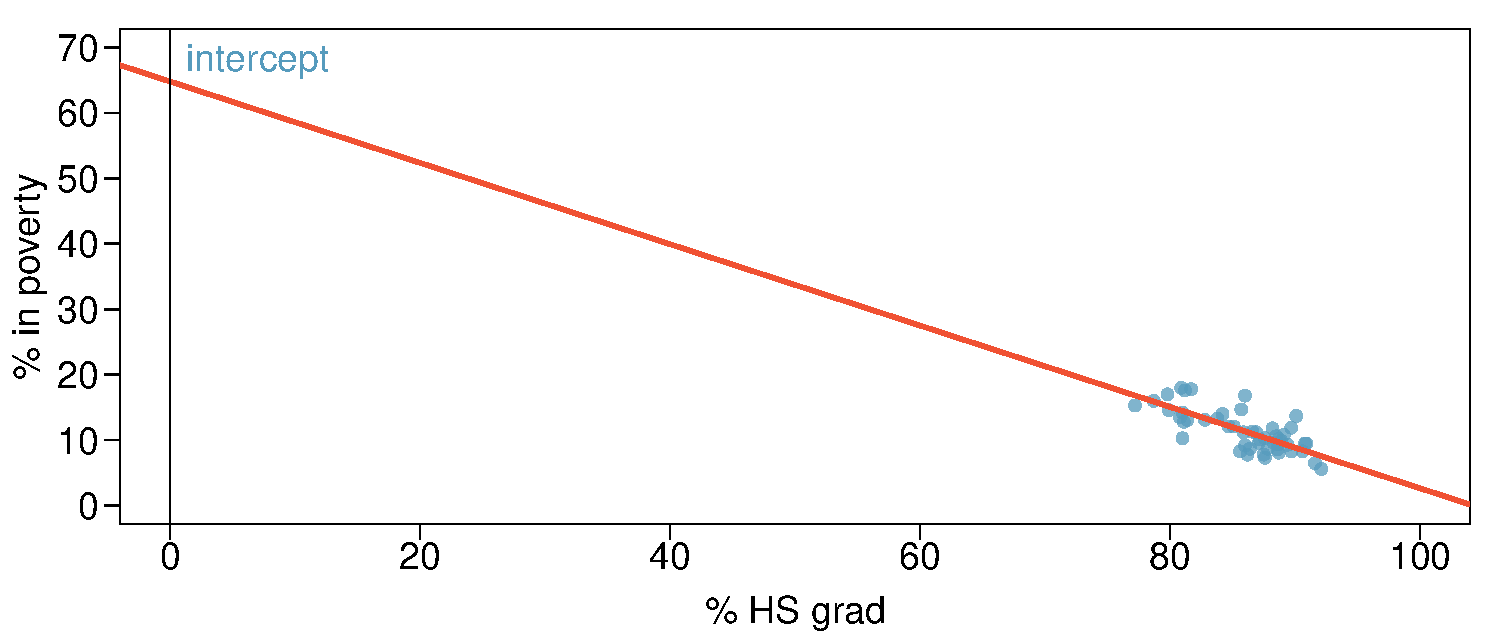
\includegraphics[width=0.75\linewidth]{8-2_least_square_reg/figures/poverty/poverty_hsgrad_line_wide}
\end{center}
}
{
\begin{align*}
b_0 &= 11.35 - (-0.62) \times 86.01 \\
&= 64.68
\end{align*}
}

\end{frame}

%%%%%%%%%%%%%%%%%%%%%%%%%%%%%%%%%%

\begin{frame}
\frametitle{}

\pq{切片の正しい解釈はどれか？}

\begin{enumerate}[(a)]
\item 高校卒業率が1\%ポイント上昇するごとに、貧困率は平均的に64.68\%増加すると予測される。
\item 高校卒業率が1\%ポイント低下するごとに、貧困率は平均的に64.68\%増加すると予測される。
\item 高校卒業者がいない場合、住民の64.68\%が貧困ライン以下で生活する。
\solnMult{高校卒業者がいない州では、住民の平均64.68\%が貧困ライン以下で生活すると予測される。}
\item 高校卒業者がいない州では、貧困率は平均的に64.68\%増加すると予測される。
\end{enumerate}

\end{frame}

%%%%%%%%%%%%%%%%%%%%%%%%%%%%%%%%%%%

\begin{frame}
\frametitle{切片についての補足}

データセットには高校卒業者が一人もいない州は存在しないため、切片はあまり意味を持たず、有用でもなく、切片の予測値がデータの大部分から大きく離れているため信頼性も低い。

\begin{center}
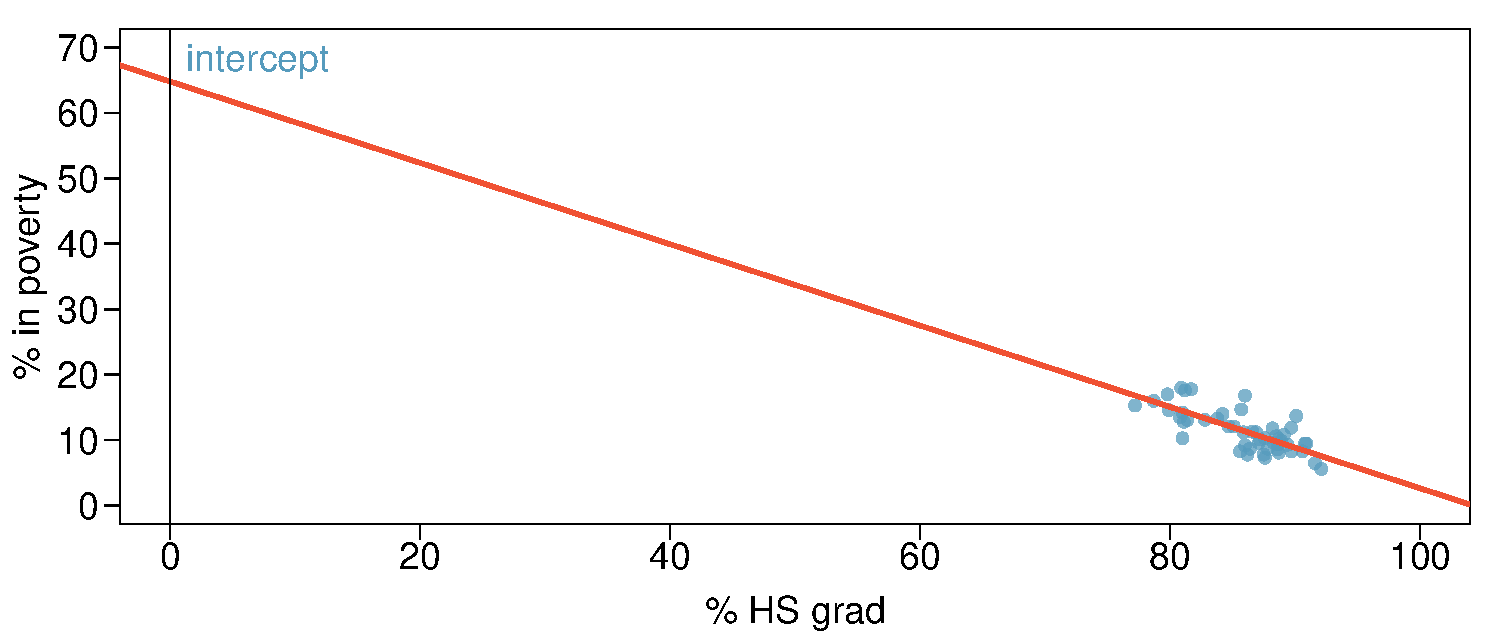
\includegraphics[width=\textwidth]{8-2_least_square_reg/figures/poverty/poverty_hsgrad_line_wide}
\end{center}

\end{frame}

%%%%%%%%%%%%%%%%%%%%%%%%%%%%%%%%%%

\begin{frame}
\frametitle{回帰直線}

\[ \widehat{\%~in~poverty} = 64.68 - 0.62~\%~HS~grad \]

\begin{center}

\includegraphics[width=0.7\textwidth]{8-2_least_square_reg/figures/poverty/poverty_hsgrad_line}
\end{center}

\end{frame}

%%%%%%%%%%%%%%%%%%%%%%%%%%%%%%%%%%

\subsection{まとめ：傾きと切片の解釈}

%%%%%%%%%%%%%%%%%%%%%%%%%%%%%%%%%%%

\begin{frame}
\frametitle{傾きと切片の解釈}

\twocol{0.5}{0.5}{
\begin{itemize}

\item \hl{切片：} $x = 0$のとき、$y$は切片に等しいと予測される。\\

$\:$ \\

\item \hl{傾き：} $x$が1単位増加するごとに、$y$は平均的に傾きの分だけ増加／減少すると予測される。

\end{itemize}
}
{
\begin{center}
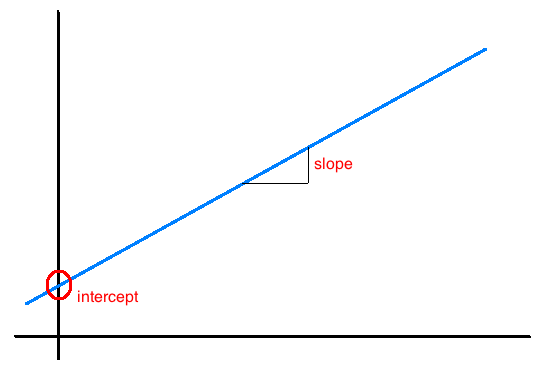
\includegraphics[width=\textwidth]{8-2_least_square_reg/figures/diagram}
\end{center}
}

\vspace{1cm}

\Note{これらの記述は、研究が無作為化比較実験でない限り、因果関係を意味しない。}

\end{frame}


%%%%%%%%%%%%%%%%%%%%%%%%%%%%%%%%%%

\subsection{予測と外挿}

%%%%%%%%%%%%%%%%%%%%%%%%%%%%%%%%%%


\begin{frame}
\frametitle{予測}

\begin{itemize}

\item 線形モデルを用いて、説明変数の特定の値に対する目的変数の値を予測することを\hl{予測}と呼ぶ。線形モデルの式に$x$の値を代入するだけでよい。

\item 予測値には不確かさが伴う。

\end{itemize}

\begin{center}
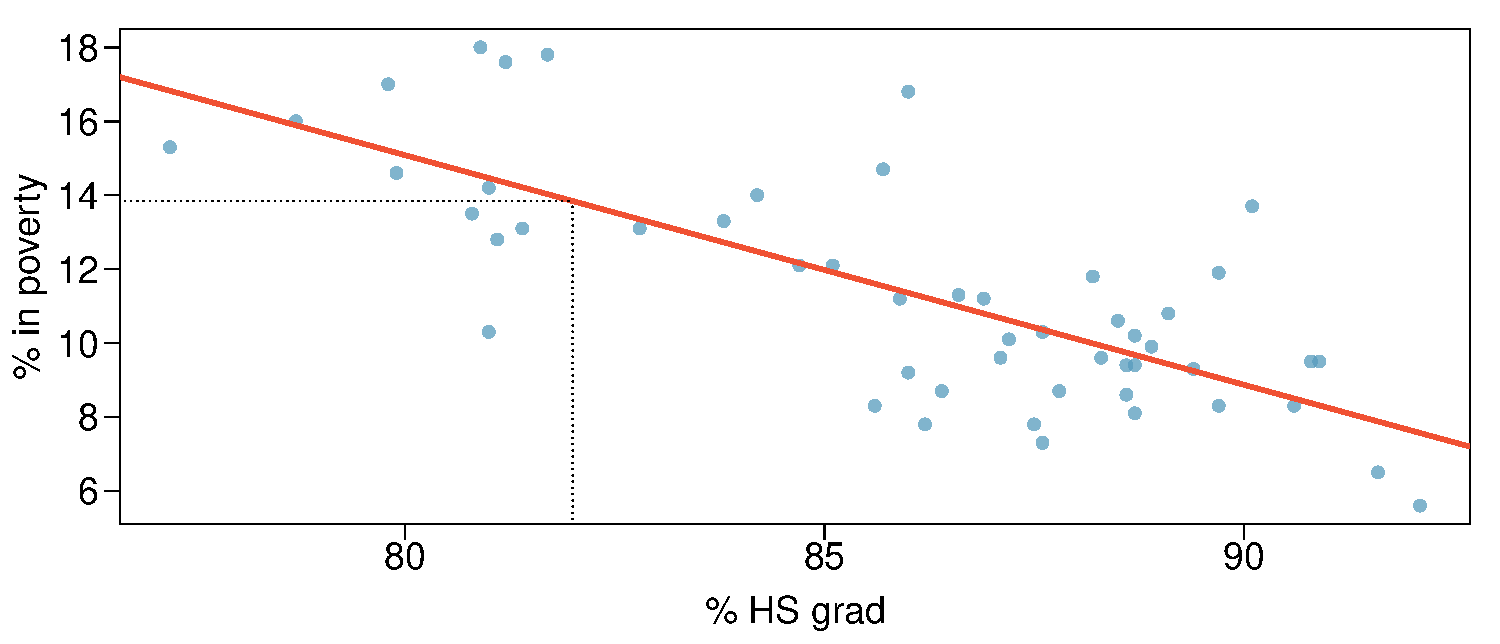
\includegraphics[width=0.9\textwidth]{8-2_least_square_reg/figures/poverty/poverty_hsgrad_pred}
\end{center}

\end{frame}

%%%%%%%%%%%%%%%%%%%%%%%%%%%%%%%%%%

\begin{frame}
\frametitle{外挿}

\begin{itemize}

\item モデルの推定を元のデータの範囲外の値に適用することを\hl{外挿}と呼ぶ。

\item 切片が外挿になる場合もある。

\end{itemize}

\begin{center}
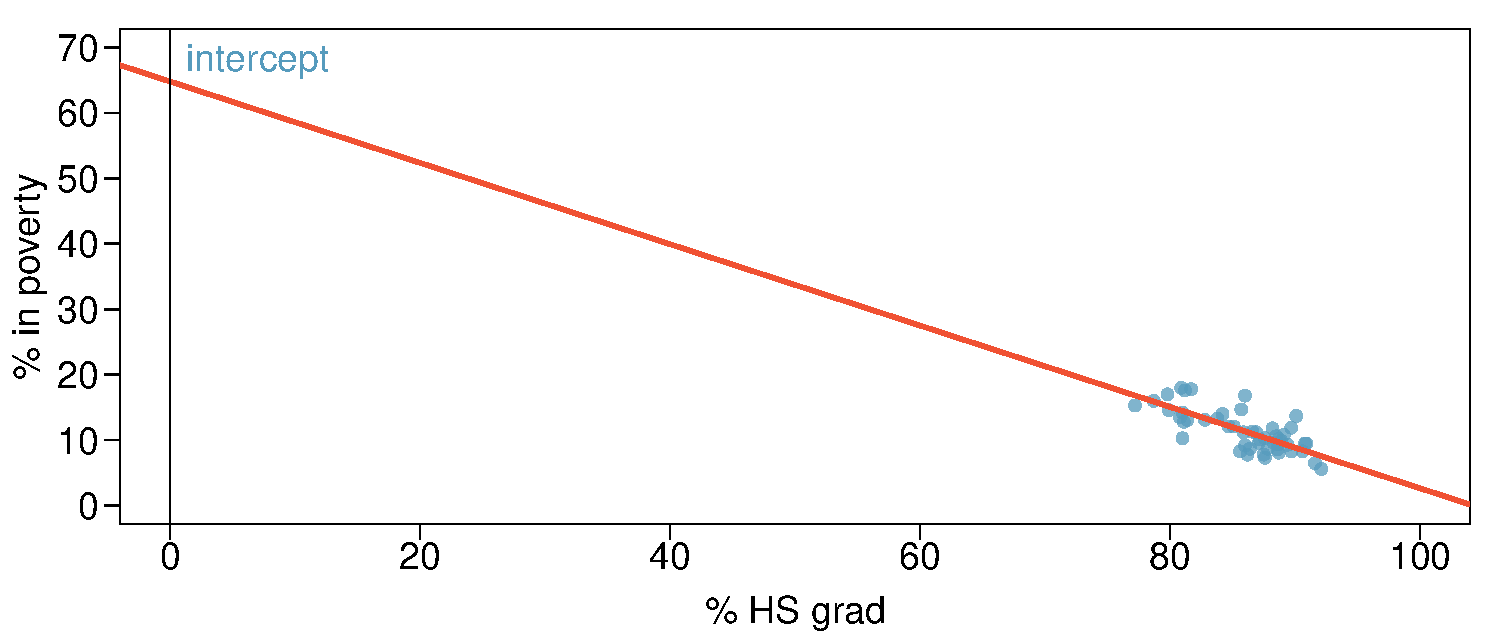
\includegraphics[width=\textwidth]{8-2_least_square_reg/figures/poverty/poverty_hsgrad_line_wide}
\end{center}

\end{frame}

%%%%%%%%%%%%%%%%%%%%%%%%%%%%%%%%%%

\begin{frame}
\frametitle{外挿の例}

\begin{center}
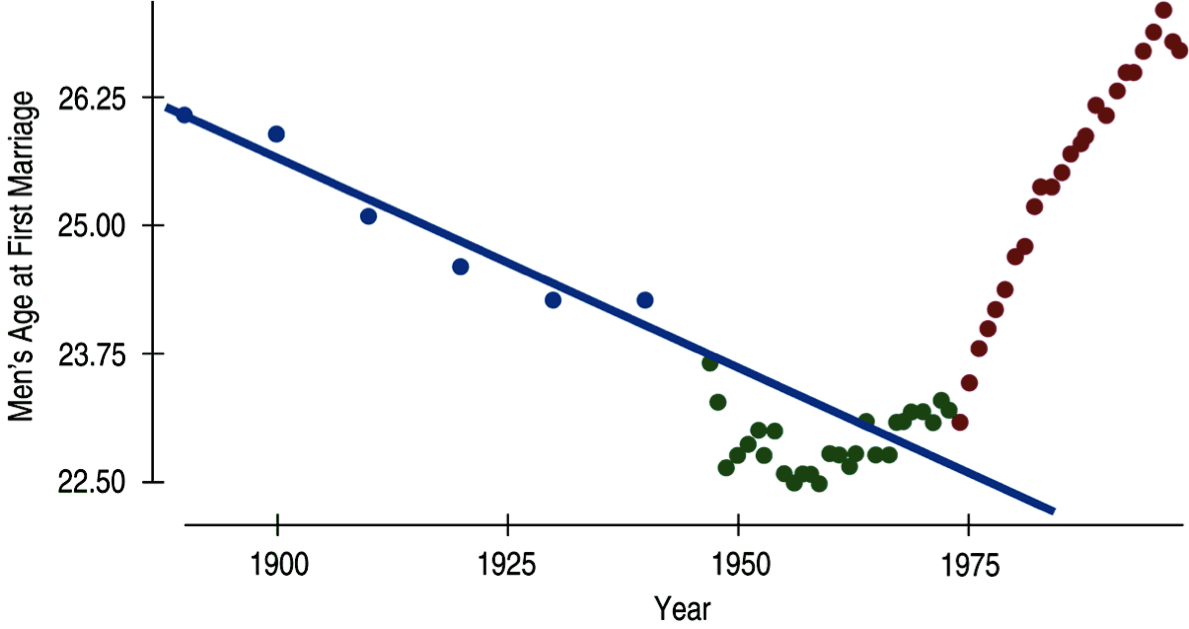
\includegraphics[width=\textwidth]{8-2_least_square_reg/figures/extrapolation}
\end{center}

\end{frame}

%%%%%%%%%%%%%%%%%%%%%%%%%%%%%%%%%%

\begin{frame}
\frametitle{外挿の例}

\begin{center}
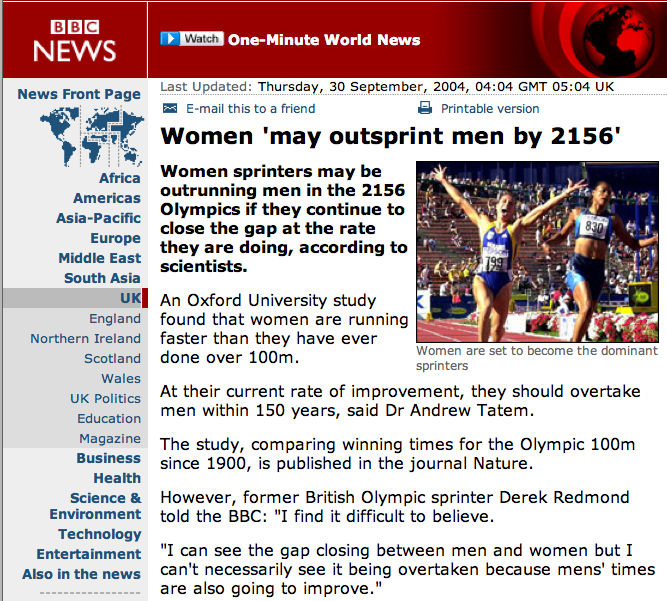
\includegraphics[width=0.7\textwidth]{8-2_least_square_reg/figures/womenOutsprintBBC}
\end{center}

\end{frame}

%%%%%%%%%%%%%%%%%%%%%%%%%%%%%%%%%%

\begin{frame}
\frametitle{外挿の例}

\begin{center}
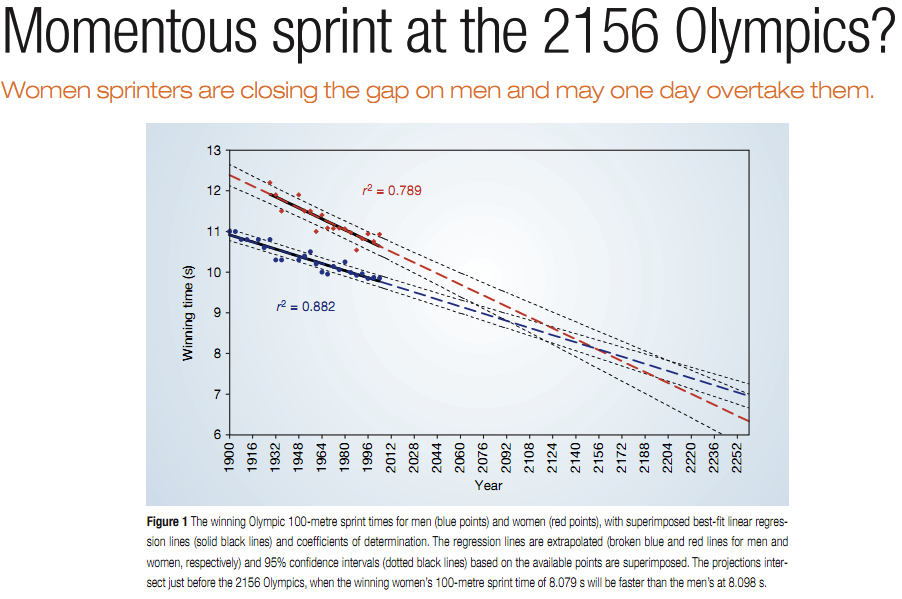
\includegraphics[width=\textwidth]{8-2_least_square_reg/figures/womenOutsprint}
\end{center}

\end{frame}

%%%%%%%%%%%%%%%%%%%%%%%%%%%%%%%%%%

\subsection{$R^2$による当てはまりの強さの記述}

%%%%%%%%%%%%%%%%%%%%%%%%%%%%%%%%%%%

\begin{frame}
\frametitle{決定係数$R^2$}

\begin{itemize}

\item 線形モデルの当てはまりの強さは、通常\mathhl{R^2}（決定係数）を用いて評価する。

\item $R^2$は相関係数の二乗として計算される。

\item 目的変数のばらつきのうち、モデルで説明できる割合を示す。

\item 残りのばらつきは、モデルに含まれていない変数またはデータの固有のランダム性によって説明される。

\item ここで扱っているモデルでは、$R^2 = (-0.75)^2 = 0.56$である。

\end{itemize}

\end{frame}

%%%%%%%%%%%%%%%%%%%%%%%%%%%%%%%%%%

\begin{frame}
\frametitle{$R^2$の解釈}

\pq{{\small $R = -0.75$、$R^2 = 0.56$の正しい解釈はどれか？}}

\twocol{0.65}{0.35}{
\begin{enumerate}[(a)]

\item 51州における高校卒業率のばらつきの56\%はモデルで説明できる。

\solnMult{51州における貧困率のばらつきの56\%はモデルで説明できる。}

\item 高校卒業率が貧困率を正しく予測できる割合は56\%である。

\item 51州における貧困率のばらつきの75\%はモデルで説明できる。

\end{enumerate}
}{
\begin{center}

\includegraphics[width=\textwidth]{8-2_least_square_reg/figures/poverty/poverty_hsgrad}
\end{center}
}

\end{frame}

%%%%%%%%%%%%%%%%%%%%%%%%%%%%%%%%%%

%%%%%%%%%%%%%%%%%%%%%%%%%%%%%%%%%%%%

\section{線形回帰における外れ値の種類}

%%%%%%%%%%%%%%%%%%%%%%%%%%%%%%%%%%%%

\begin{frame}
\frametitle{外れ値の種類}

\twocol{0.5}{0.5}
{
\dq{この散布図において、外れ値は最小二乗直線にどのような影響を与えているか？}

この問いに答えるために、外れ値がある場合とない場合の回帰直線がどうなるかを考える。外れ値がない場合、回帰直線はより急な傾きになり、大きな観測値の集まりに近くなる。外れ値がある場合、直線は上方に引っ張られ、大きな観測値の集まりの一部から遠ざかる。
}
{
\begin{center}
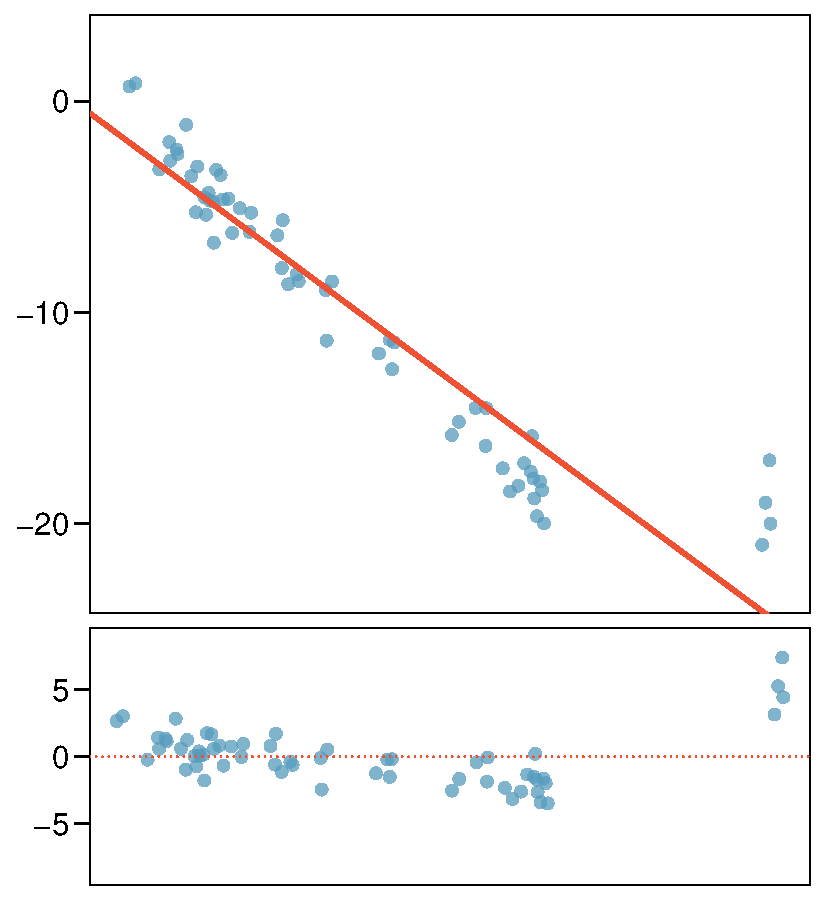
\includegraphics[width=\textwidth]{8-3_outliers/figures/outlierPlots/out4}
\end{center}
}

\end{frame}

%%%%%%%%%%%%%%%%%%%%%%%%%%%%%%%%%%%

\begin{frame}
\frametitle{外れ値の種類}

\twocol{0.4}{0.6}
{
\dq{この散布図において、外れ値は最小二乗直線にどのような影響を与えているか？} \\
\soln{外れ値がない場合、$x$と$y$の間に明らかな関係は見られない。}
}
{
\begin{center}
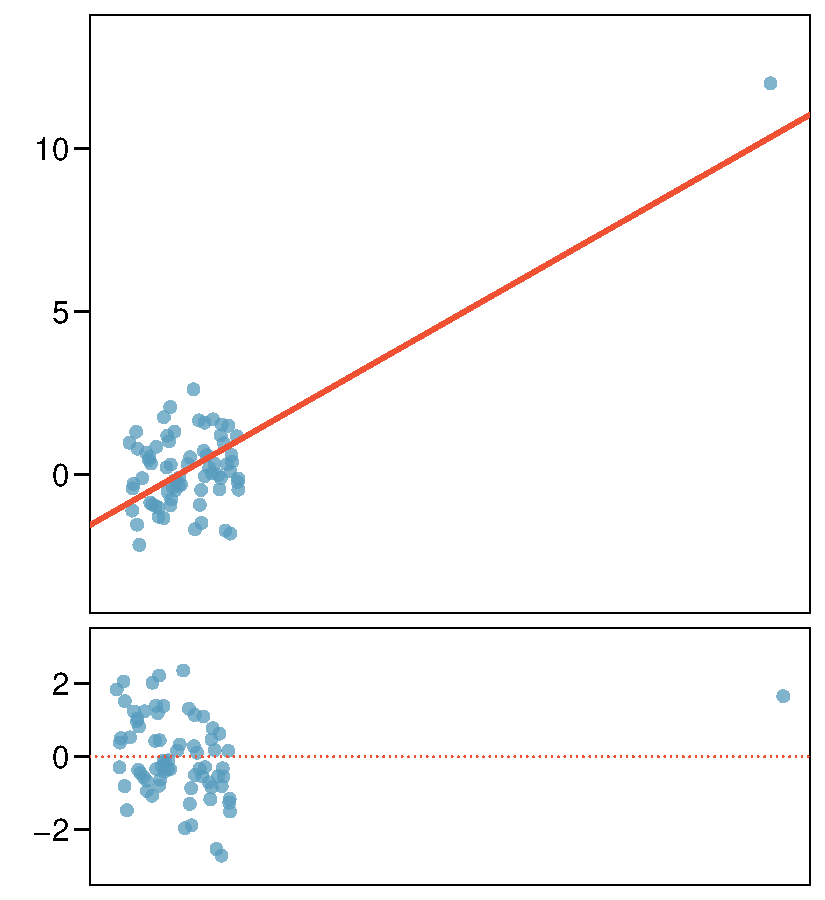
\includegraphics[width=\textwidth]{8-3_outliers/figures/outlierPlots/out5}
\end{center}
}

\end{frame}

%%%%%%%%%%%%%%%%%%%%%%%%%%%%%%%%%%%

\begin{frame}
\frametitle{用語}

\begin{itemize}

\item \hl{外れ値}とは、点の集まりから離れた位置にある点のことである。

\item 点の集まりの中心から水平方向に離れた外れ値を\hl{高レバレッジ点}（high leverage points）と呼ぶ。

\item 回帰直線の\underline{傾き}に実際に影響を与える高レバレッジ点を\hl{影響点}（influential points）と呼ぶ。

\item ある点が影響点かどうかを判断するには、その点がある場合とない場合の回帰直線を視覚的に比較する。直線の傾きが大きく変わる場合、その点は影響点である。大きく変わらない場合は影響点ではない。

\end{itemize}

\end{frame}

%%%%%%%%%%%%%%%%%%%%%%%%%%%%%%%%%%%

\begin{frame}
\frametitle{影響点}

星団CYG OB1に属する47個の星について、表面温度の対数と光度の対数のデータが得られている。

\twocol{0.7}{0.3}
{
\begin{center}
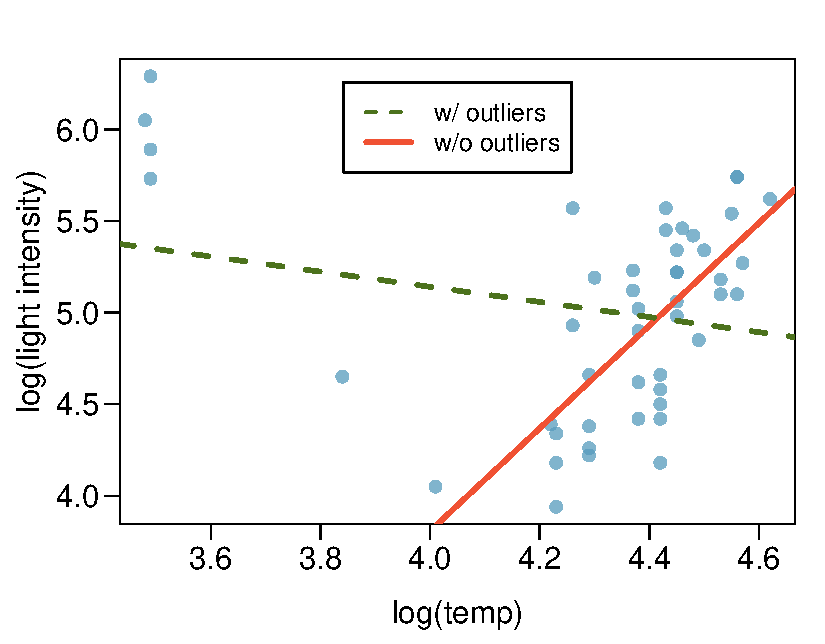
\includegraphics[width=\textwidth]{8-3_outliers/figures/stars/star}
\end{center}
}
{
\begin{center}
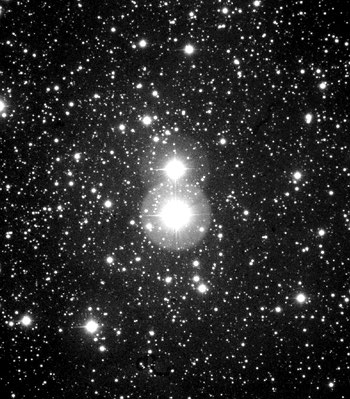
\includegraphics[width=\textwidth]{8-3_outliers/figures/stars/cyg}
\end{center}
}

\end{frame}

%%%%%%%%%%%%%%%%%%%%%%%%%%%%%%%%%%%

\begin{frame}
\frametitle{外れ値の種類}

\twocol{0.4}{0.6}
{
\pq{この外れ値を最もよく表す記述はどれか？}
\begin{enumerate}[(a)]
\item 影響点
\solnMult{高レバレッジ点}
\item 上記のいずれでもない
\item 外れ値はない
\end{enumerate}
}
{
\begin{center}
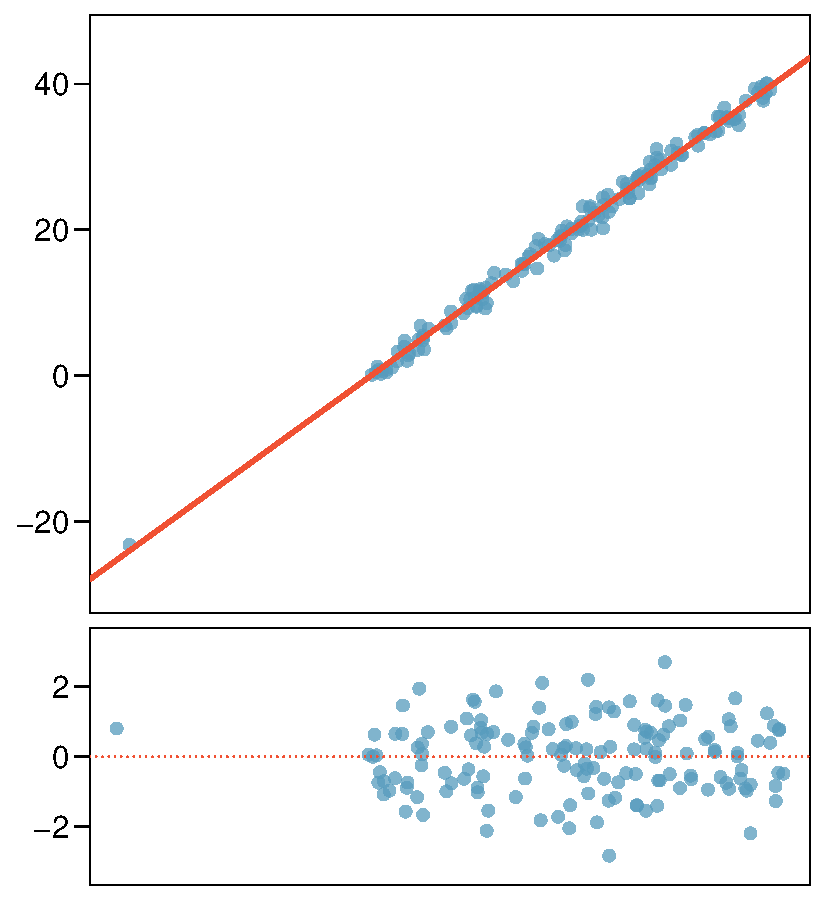
\includegraphics[width=\textwidth]{8-3_outliers/figures/outlierPlots/out6}
\end{center}
}

\end{frame}

%%%%%%%%%%%%%%%%%%%%%%%%%%%%%%%%%%%

\begin{frame}
\frametitle{外れ値の種類}

\twocol{0.4}{0.6}
{
\dq{この外れ値は回帰直線の傾きに影響を与えているか？}
\soln{あまり影響していない…}

}
{
\begin{center}
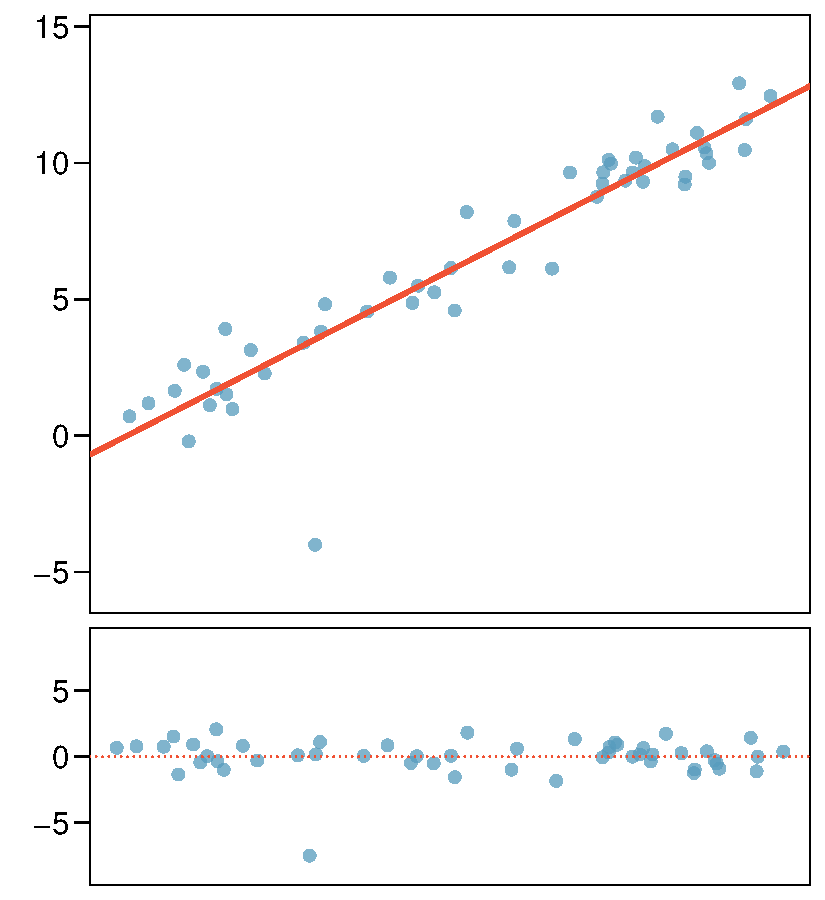
\includegraphics[width=\textwidth]{8-3_outliers/figures/outlierPlots/out1}
\end{center}
}

\end{frame}

%%%%%%%%%%%%%%%%%%%%%%%%%%%%%%%%%%%

\begin{frame}
\frametitle{まとめ}

\pq{次のうち\underline{正しい}記述はどれか？}

\begin{enumerate}[(a)]
\item 影響点は常に回帰直線の切片を変化させる。
\item 影響点は常に$R^2$を低下させる。
\item 低レバレッジ点の方が高レバレッジ点よりも影響点になりやすい。
\item データセットに影響点が含まれる場合、説明変数と目的変数の関係は常に非線形である。
\solnMult{上記のいずれも正しくない。}
\end{enumerate}

\end{frame}

%%%%%%%%%%%%%%%%%%%%%%%%%%%%%%%%%%%

\begin{frame}
\frametitle{まとめ（続き）}

\vspace{-1cm}

\twocol{0.5}{0.5}
{
\begin{center}
\[ R = 0.08, R^2 = 0.0064 \]
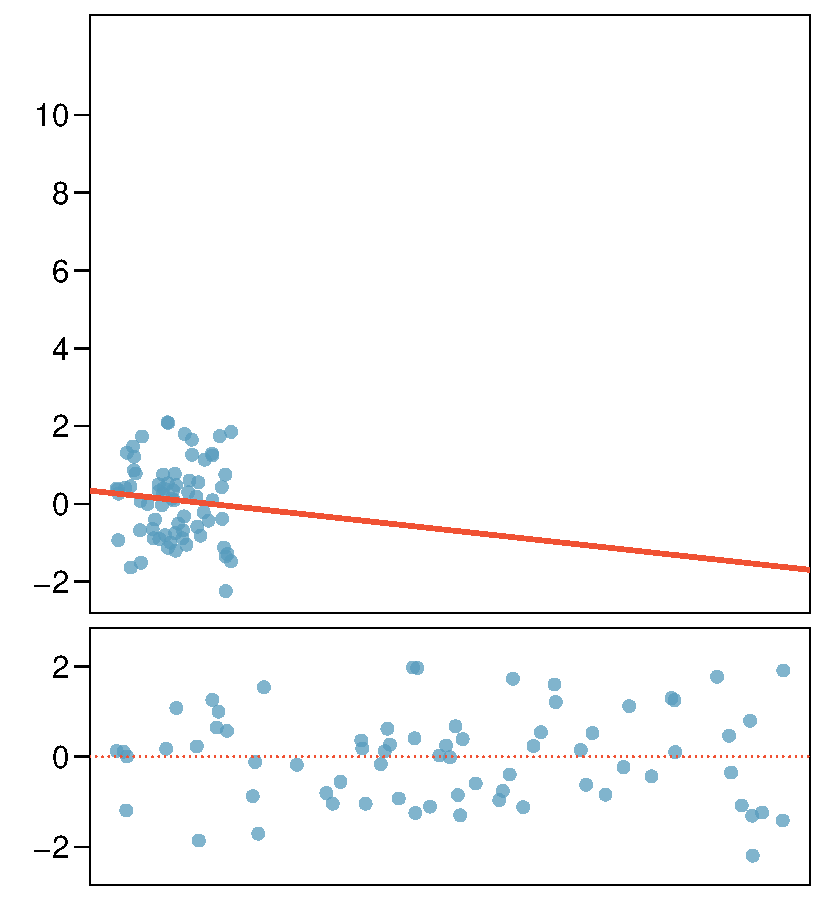
\includegraphics[width=\textwidth]{8-3_outliers/figures/outlierPlots/out5-1}
\end{center}
}
{
\begin{center}
\[ R = 0.79, R^2 = 0.6241 \]
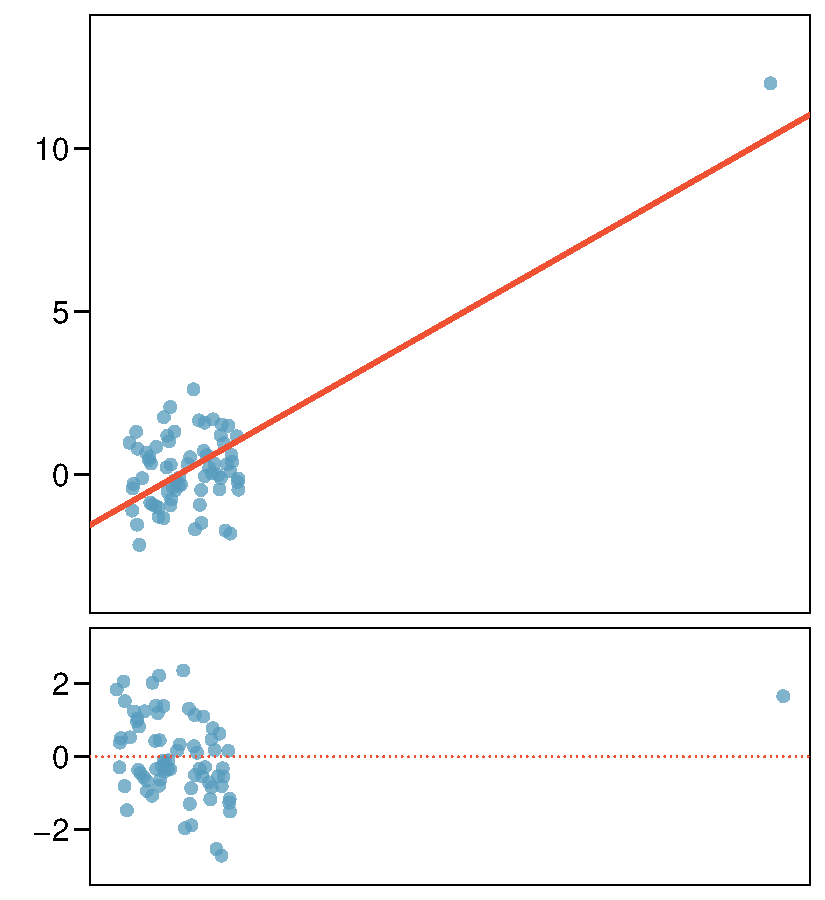
\includegraphics[width=\textwidth]{8-3_outliers/figures/outlierPlots/out5}
\end{center}
}

\end{frame}

%%%%%%%%%%%%%%%%%%%%%%%%%%%%%%%%%%%%

\section{線形回帰の推測}

%%%%%%%%%%%%%%%%%%%%%%%%%%%%%%%%%%%%

\subsection{ソフトウェアの回帰出力の読み方}

%%%%%%%%%%%%%%%%%%%%%%%%%%%%%%%%%%%

\begin{frame}
\frametitle{遺伝か環境か？}

{\small 1966年、Cyril Burtは「知能の差異の遺伝的決定：一緒に育てられた双子と別々に育てられた双子の研究」という論文を発表した。データは、一卵性双生児27組（代表的な無作為標本と仮定）のIQスコアで構成されており、一方は養親に、もう一方は実の親に育てられた。}

\begin{center}
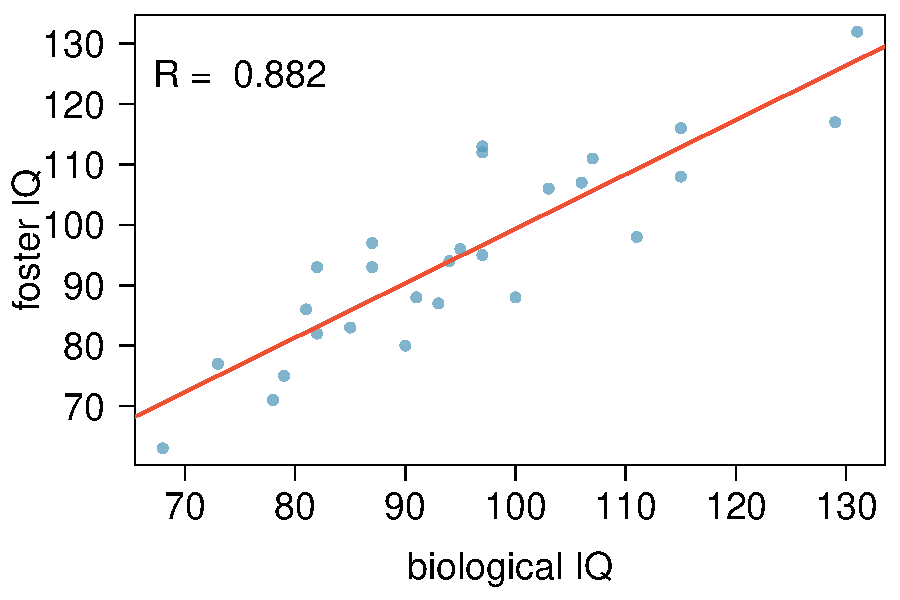
\includegraphics[width=0.7\textwidth]{8-4_inf_lin_reg/figures/twins/twins_IQ}
\end{center}

\end{frame}

%%%%%%%%%%%%%%%%%%%%%%%%%%%%%%%%%%%

\begin{frame}[fragile]
\frametitle{}

\pq{次のうち\underline{誤っている}記述はどれか？}

{\footnotesize
\begin{verbatim}
Coefficients:
                 Estimate Std. Error t value Pr(>|t|)
(Intercept)       9.20760    9.29990   0.990    0.332
bioIQ             0.90144    0.09633   9.358  1.2e-09

Residual standard error: 7.729 on 25 degrees of freedom
Multiple R-squared: 0.7779,	Adjusted R-squared: 0.769
F-statistic: 87.56 on 1 and 25 DF,  p-value: 1.204e-09
\end{verbatim}
}

\begin{enumerate}[(a)]
\item 実の親に育てられた双子のIQが10ポイント高い場合、養親に育てられた双子のIQは平均的に9ポイント高いと関連づけられる。
\solnMult{養親に育てられた双子のIQの約78\%はモデルで正確に予測できる。}
\item 線形モデルは$\widehat{fosterIQ} = 9.2 + 0.9 \times bioIQ$である。
\item 平均より高いIQを持つ養育双子は、平均より高いIQを持つ実親双子と対応している傾向がある。
\end{enumerate}

\end{frame}

%%%%%%%%%%%%%%%%%%%%%%%%%%%%%%%%%%%

\begin{frame}
\frametitle{傾きの検定}

\pq{出生時に引き離されたすべての双子の代表的な標本としてこの27組を想定した場合、実の親に育てられた双子のIQが養親に育てられた双子のIQの有意な予測因子であるかどうかを検定するための適切な仮説はどれか？}

\begin{enumerate}[(a)]
\item \mathhl{H_0:} $b_0 = 0$; \mathhl{H_A:} $b_0 \ne 0$
\item \mathhl{H_0:} $\beta_0 = 0$; \mathhl{H_A:} $\beta_0 \ne 0$
\item \mathhl{H_0:} $b_1 = 0$; \mathhl{H_A:} $b_1 \ne 0$
\solnMult{\mathhl{H_0:} $\beta_1 = 0$; \mathhl{H_A:} $\beta_1 \ne 0$}
\end{enumerate}

\end{frame}

%%%%%%%%%%%%%%%%%%%%%%%%%%%%%%%%%%%

\begin{frame}
\frametitle{傾きの検定（続き）}

{\footnotesize
\begin{center}
\begin{tabular}{rrrrr}
  \hline
 & Estimate & Std. Error & t value & Pr($>$$|$t$|$) \\
  \hline
(Intercept) & 9.2076 & 9.2999 & 0.99 & 0.3316 \\
  bioIQ & 0.9014 & 0.0963 & 9.36 & 0.0000 \\
   \hline
\end{tabular}
\end{center}
}

\begin{itemize}

\item 回帰の推測では常に$t$検定を用いる。$\:$ \\

\Remember{検定統計量 $T = \frac{\text{点推定量} - \text{帰無値}}{SE}$}

\item 点推定量 = $b_1$は観測された傾きである。

\item $SE_{b_1}$は傾きに関連する標準誤差である。

\item 傾きに関連する自由度は$df = n - 2$であり、$n$は標本サイズである。$\:$ \\
\Remember{推定するパラメータ1つにつき自由度を1つ失う。単回帰では$\beta_0$と$\beta_1$の2つのパラメータを推定するため、$df = n - 2$となる。}

\end{itemize}

\end{frame}

%%%%%%%%%%%%%%%%%%%%%%%%%%%%%%%%%%%

\begin{frame}
\frametitle{傾きの検定（続き）}

{\small
\begin{center}
\begin{tabular}{rrrrr}
  \hline
 & Estimate & Std. Error & t value & Pr($>$$|$t$|$) \\
  \hline
(Intercept) &  9.2076 & 9.2999 & 0.99 & 0.3316 \\
  bioIQ & \orange{0.9014}  &   \green{0.0963} & \orange{9.36} & \textcolor{blue}{0.0000} \\
   \hline
\end{tabular}
\end{center}
}

\begin{eqnarray*}
T &=& \frac{\orange{0.9014} - 0}{\green{0.0963}} = \orange{9.36} \\
df &=& 27 - 2 = 25 \\
p\text{値} &=& P(|T| > \orange{9.36}) < \textcolor{blue}{0.01}
\end{eqnarray*}

\end{frame}

%%%%%%%%%%%%%%%%%%%%%%%%%%%%%%%%%%%

\begin{frame}
\frametitle{LA地区における大学卒業率とヒスパニック系住民割合}

\dq{LAの100の郵便番号地域の標本において、大学卒業率とヒスパニック系住民割合の関係について何が言えるか？}

\begin{center}
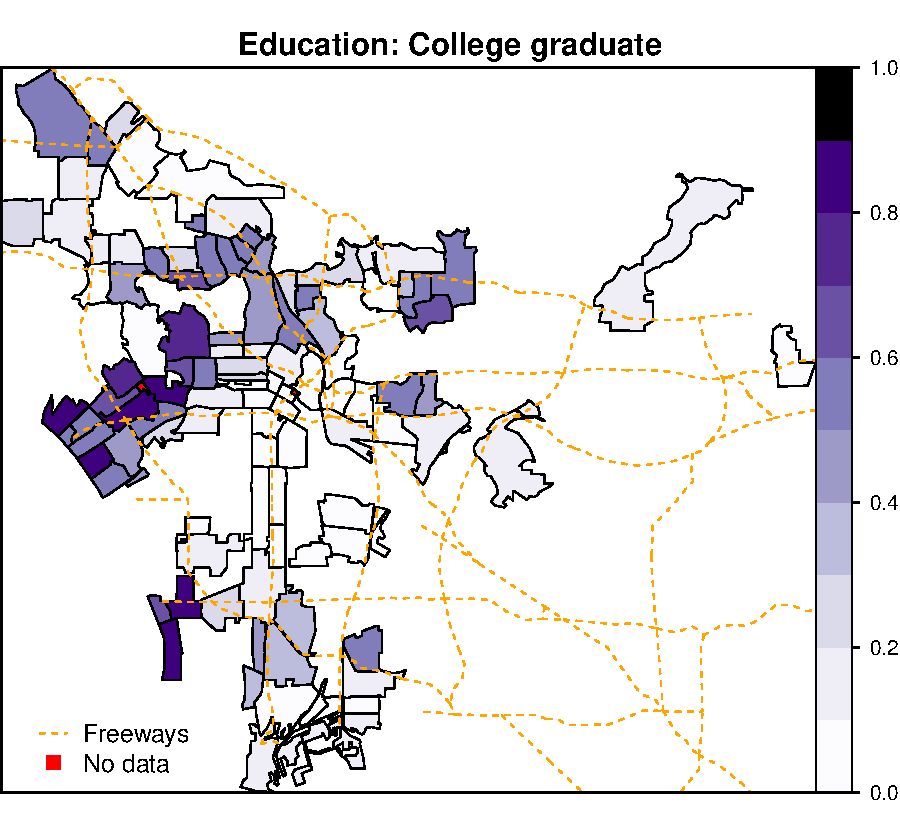
\includegraphics[width=0.46\textwidth]{8-4_inf_lin_reg/figures/la/Prop_EduHigherThan16th}~~~~
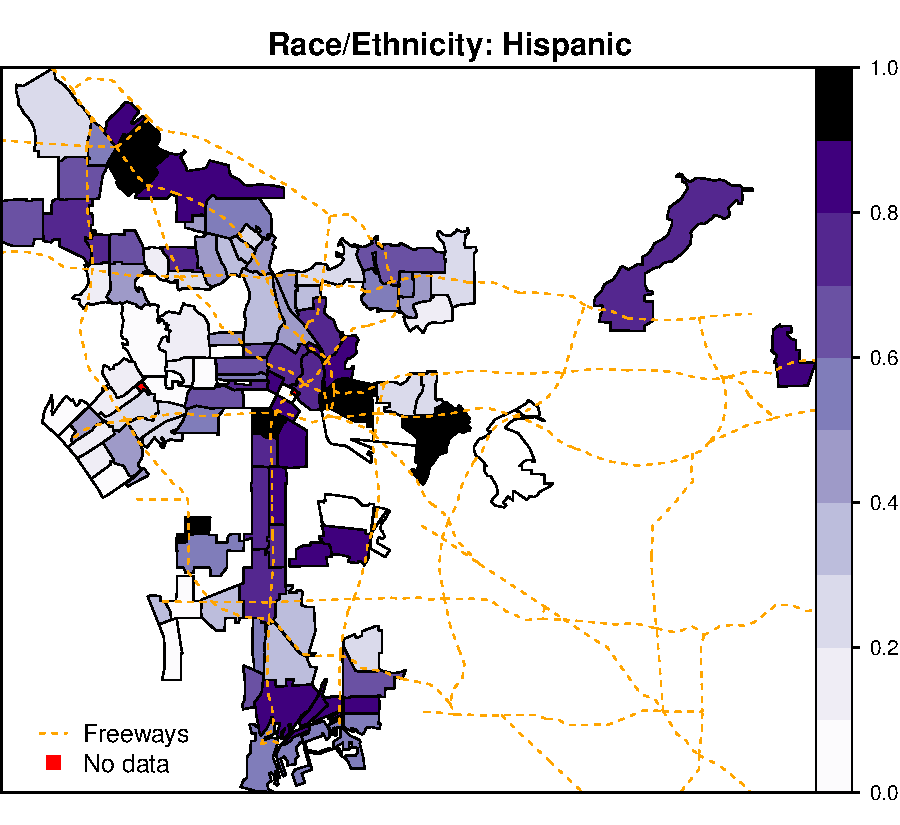
\includegraphics[width=0.46\textwidth]{8-4_inf_lin_reg/figures/la/Prop_RaceEthHispanic}
\end{center}

\end{frame}

%%%%%%%%%%%%%%%%%%%%%%%%%%%%%%%%%%%

\begin{frame}
\frametitle{LA地区における大学卒業率とヒスパニック系住民割合（別の視点）}

\dq{LAの100の郵便番号地域の標本において、大学卒業率とヒスパニック系住民割合の関係について何が言えるか？}

\begin{center}
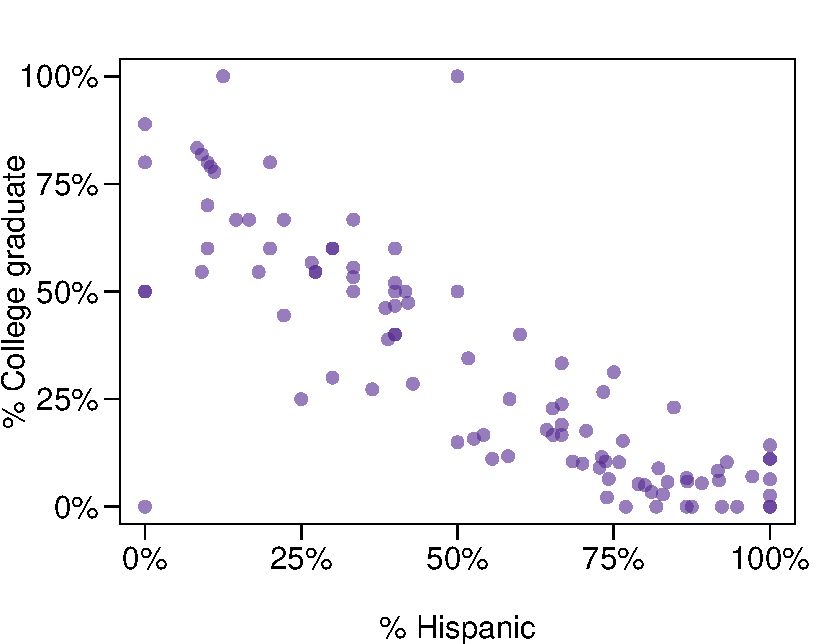
\includegraphics[width=0.7\textwidth]{8-4_inf_lin_reg/figures/la/la}
\end{center}

\end{frame}

%%%%%%%%%%%%%%%%%%%%%%%%%%%%%%%%%%%

\begin{frame}
\frametitle{LA地区における大学卒業率とヒスパニック系住民割合：線形モデル}

\pq{傾きの最もよい解釈はどれか？}

{\small
\begin{center}
\begin{tabular}{rrrrr}
  \hline
 & Estimate & Std. Error & t value & Pr($>$$|$t$|$) \\
  \hline
(Intercept) & 0.7290 & 0.0308 & 23.68 & 0.0000 \\
 \%Hispanic & -0.7527 & 0.0501 & -15.01 & 0.0000 \\
   \hline
\end{tabular}
\end{center}
}

\begin{enumerate}[(a)]
\item LA地区の郵便番号地域でヒスパニック系住民が1\%増加すると、大学卒業率は75\%低下する。
\solnMult{LA地区の郵便番号地域でヒスパニック系住民が1\%増加すると、大学卒業率は0.75\%低下する。}
\item ヒスパニック系住民が1\%追加されるごとに、LA地区の郵便番号地域の大学卒業率は0.75\%低下する。
\item ヒスパニック系住民がいない郵便番号地域では、大学卒業率は75\%と予測される。
\end{enumerate}

\end{frame}

%%%%%%%%%%%%%%%%%%%%%%%%%%%%%%%%%%%

\begin{frame}
\frametitle{LA地区における大学卒業率とヒスパニック系住民割合：線形モデル}

\dq{このデータはLA地区の郵便番号地域においてヒスパニック系住民割合と大学卒業率の間に統計的に有意な関係があることの説得力ある証拠を提供しているか？}

{\small
\begin{center}
\begin{tabular}{rrrrr}
  \hline
 & Estimate & Std. Error & t value & Pr($>$$|$t$|$) \\
  \hline
(Intercept) & 0.7290 & 0.0308 & 23.68 & 0.0000 \\
  hispanic & -0.7527 & 0.0501 & -15.01 & 0.0000 \\
   \hline
\end{tabular}
\end{center}
}
\soln{はい。ヒスパニック系住民割合のp値が小さく、傾きパラメータが0と異なることの説得力ある証拠をデータが提供していることを示している。}

$\:$ \\

\dq{これらの郵便番号地域が無作為に選択されていない場合、このp値はどの程度信頼できるか？}
\soln{あまり信頼できない…}

\end{frame}

%%%%%%%%%%%%%%%%%%%%%%%%%%%%%%%%%%%

\subsection{傾きの信頼区間}

%%%%%%%%%%%%%%%%%%%%%%%%%%%%%%%%%%%

\begin{frame}
\frametitle{傾きの信頼区間}

\pq{{\small 信頼区間は$\text{点推定量} \pm ME$として計算され、単回帰における傾きの自由度は$n - 2$であることを思い出してほしい。27組の双子の観測に基づくモデルにおいて、傾きパラメータの95\%信頼区間として正しいものはどれか？}}

{\footnotesize
\begin{center}
\begin{tabular}{rrrrr}
  \hline
 & Estimate & Std. Error & t value & Pr($>$$|$t$|$) \\
  \hline
(Intercept) & 9.2076 & 9.2999 & 0.99 & 0.3316 \\
  bioIQ & 0.9014 & 0.0963 & 9.36 & 0.0000 \\
   \hline
\end{tabular}
\end{center}
}

\vspace{-0.5cm}

\twocol{0.4}{0.6}
{
\begin{enumerate}[(a)]
\item $9.2076 \pm 1.65 \times 9.2999$
\solnMult{$0.9014 \pm 2.06 \times 0.0963$}
\item $0.9014 \pm 1.96 \times 0.0963$
\item $9.2076 \pm 1.96 \times 0.0963$
\end{enumerate}
}
{
\soln{\onslide<2->{\orange{
\begin{eqnarray*}
n &=& 27 \qquad df = 27 - 2 = 25 \\
95\%:~t^\star_{25} &=& 2.06 \\
0.9014 &\pm& 2.06 \times 0.0963 \\
(0.7 &,& 1.1)
\end{eqnarray*}
}}}}

\end{frame}

%%%%%%%%%%%%%%%%%%%%%%%%%%%%%%%%%%%

\begin{frame}
\frametitle{まとめ}

\begin{itemize}

\item 単回帰モデルの傾きに対する推測：
\begin{itemize}
\item 仮説検定：
\[ T = \frac{b_1 - \text{帰無値}}{SE_{b_1}} \qquad df = n - 2 \]
\item 信頼区間：
\[ b_1 \pm t^\star_{df = n - 2} SE_{b_1} \]
\end{itemize}

\item 帰無値は、説明変数と目的変数の間に\hl{何らかの}関係があるかを確認するため、通常0に設定される。

\item 回帰出力には$b_1$、$SE_{b_1}$、および帰無値が0の場合の傾きの$t$検定の\hl{両側}p値が含まれる。

\item 切片の推測を行うことはほとんどないため、傾きの推定と推測に焦点を当てる。

\end{itemize}

\end{frame}

%%%%%%%%%%%%%%%%%%%%%%%%%%%%%%%%%%%


\begin{frame}
\frametitle{注意事項}

\begin{itemize}

\item 扱っているデータの種類（無作為標本、非無作為標本、または母集団）を常に把握しておくこと。

\item すでに母集団データがある場合、統計的推測とそれに基づくp値は意味を持たない。

\item 偏った非無作為標本を使用している場合、推測の結果は信頼できない。

\item 最終的な目標は、独立した観測値を持つことである。

\end{itemize}

\end{frame}

%%%%%%%%%%%%%%%%%%%%%%%%%%%%%%%%%%%



%%%%%%%%%%%%%%%%%%%%%%%%%%%%%%%%%%%%
% ドキュメント終了
%%%%%%%%%%%%%%%%%%%%%%%%%%%%%%%%%%%%

\end{document}
